\section{Introduction}
\label{sec:intro}

Large language models (LLMs) have demonstrated impressive generalization capabilities across a wide range of tasks. These AI agents rely on intelligence embedded in their pretrained parameters, and increasingly, on learning from task-specific signals, whether explicit (e.g., labeled supervision) or implicit (e.g., user interactions, feedback). A key challenge is enabling agents to continuously improve their performance and generalize to unseen domains or tasks by distilling knowledge from such signals and storing them in a reusable and interpretable form.

Traditional approaches to learning from new signals often involve updating model parameters through fine-tuning~\cite{radford2018improving, howard-ruder-2018-universal} or adaptation mechanisms such as parameter-efficient methods (e.g., LoRA adapters)~\cite{pmlr-v97-houlsby19a,hu2022lora}. While effective, these approaches incur computational cost, require retraining for every new signal or task, and often lack interpretability or controllability. Furthermore, they provide limited support for never-ending learning, where an agent must continuously adapt without retraining from scratch or storing large sets of models.

An alternative paradigm is memory-augmented learning~\cite{a27da5feb471466cb024242bf91426d3,Zhong_Guo_Gao_Ye_Wang_2024, salama-etal-2025-meminsight}, where the underlying model remains frozen, and adaptation occurs through interaction with an external memory. This memory stores relevant task knowledge, examples, demonstrations, or explanations, that can be retrieved at inference time to inform the model’s decisions. Among such approaches, in-context learning (ICL)~\cite{dong-etal-2024-survey} has emerged as a simple yet powerful mechanism, where the model is conditioned on a prompt consisting of a small number of examples (few-shot learning). 
However, directly incorporating supervised signals in the LLM context often relies on only few-shot input-output examples and tends to result in shallow pattern mimicking, due to a lack of deeper abstraction or conceptual understanding.

\begin{figure*}
    \centering
    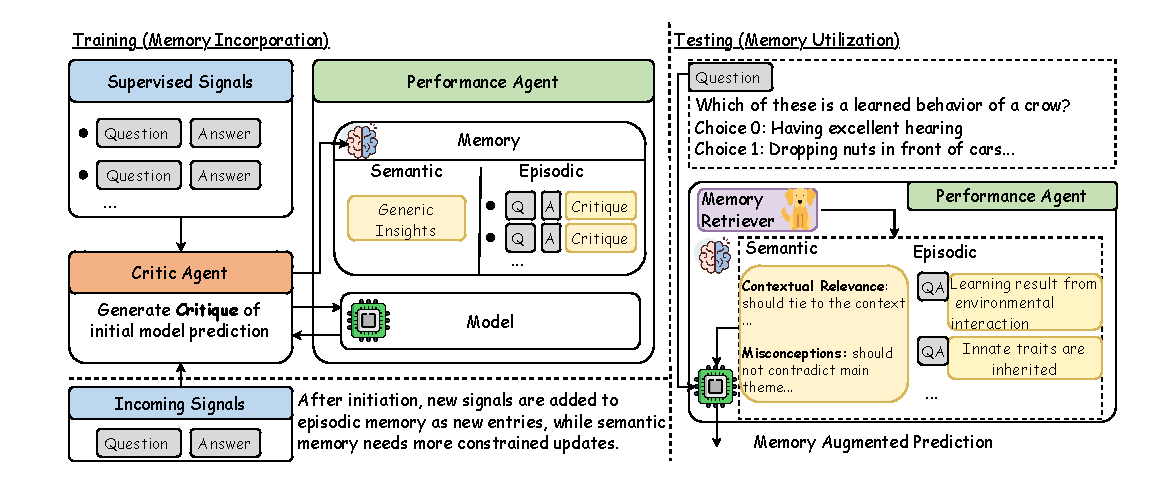
\includegraphics[width=1.0\textwidth]{figures/critique-diagram.drawio.pdf}
    \caption{Agents learn from supervised signals by incorporating them into memory. At inference time, both task-level insights (semantic memory) and context-specific information (episodic memory) can support more informed decision-making. }
    \label{fig:diagram}
\end{figure*}


Recent work ~\cite{NEURIPS2023_91edff07,yao2023react,gou2024critic,NEURIPS2023_1b44b878, zhang2025spiralsymbolicllmplanning} has highlighted the capacity of LLM agents to not only perform tasks but also critique them, generating feedback and identifying patterns of errors in their own outputs. Several notable approaches leverage self-critique, but they differ fundamentally from our objectives. Self-Refine~\cite{NEURIPS2023_91edff07} relies purely on a model iteratively refining its response to a single question using parametric knowledge, and does not produce reusable memory artifacts utilized in future predictions. CRITIC~\cite{gou2024critic} extends this iterative process by grounding self-critiques in external tool outputs, but similarly lacks the generation of reusable memories derived from gold-standard data. Reflexion~\cite{NEURIPS2023_1b44b878} approximates reinforcement learning by storing self-critiques from synthetic environments, but it relies on binary correctness signals from the environment rather than pre-labeled data and restricts memory retrieval to identical tasks, limiting its ability to generalize. In contrast to these methods, our primary differentiator is grounding critiques in gold-standard labeled data to produce reusable memory artifacts. This grounds the critiques in supervised data as a way to provide novel information to the agent, avoiding the simple reinforcement of the base LLM's parametric biases.  

Inspired by human tutoring, where feedback often includes explanations of mistakes and guidance for improvement, we explore whether such reflective insights can be distilled into reusable knowledge for future tasks. Instead of merely memorizing example responses, we hypothesize that an agent that internalizes structured feedback can develop a deeper understanding of task requirements and generalize more effectively to new examples.

In this paper, we investigate how LLM agents can effectively and continuously learn from supervised signals and deeper reasoning provided by critiques, incorporating these insights into memory. 
